% U4 WS1 -- Type B: change classification + particulate representations.
\documentclass{apchem-worksheet}

\apcunit{4}
\apcunittitle{Chemical Reactions}
\apcdoctitle{Worksheet 1 \textbullet\ Change and Representation}
\apcsubtitle{CED 4.1, 4.3, 4.4 \textbullet\ drawing counts as much as calculating here}

\begin{document}
\wsheader[Every particulate drawing must conserve atoms and charge. Label
what your circles represent --- an unlabelled diagram earns nothing.]

\problem[4.4]{Classify each as physical or chemical change and give the
particle-level reason:}
\begin{parts}
  \item Water boiling: \answerblank[7.2cm]{physical --- \ce{H2O} molecules
        separate}
  \item Copper turning green outdoors:
        \answerblank[7.7cm]{chemical --- new carbonate compound}
  \item Sugar dissolving in tea: \answerblank[7.4cm]{physical --- molecules
        disperse intact}
  \item Baking soda fizzing in vinegar:
        \answerblank[6.5cm]{chemical --- \ce{CO2} gas produced}
\end{parts}

\problem[4.4]{Dissolving \ce{NaCl} is classified as a physical change, yet
ionic bonds are disrupted. Reconcile these two statements.
\answerlines[3]{The ions are separated and hydrated, but no new substance
forms --- the same \ce{Na+} and \ce{Cl-} are present, and evaporating the
water recovers the original solid. Chemical change requires new
substances, not merely separated ones.}}

\problem[4.1]{A student mixes two clear solutions; the mixture becomes
warm and slightly cloudy.}
\begin{parts}
  \item Name two pieces of evidence suggesting a chemical reaction.
        \answerlines[2]{Temperature rise (energy released as bonds form)
        and cloudiness (a precipitate forming).}
  \item Give one alternative explanation for each observation that does
        \emph{not} require a chemical reaction.
        \answerlines[3]{Warming can accompany simple dissolving (exothermic
        hydration). Cloudiness could be undissolved solid or an immiscible
        liquid dispersing, not a new compound.}
  \item What single additional test would most strengthen the claim?
        \answerlines[2]{Filter and identify the solid --- confirming it is
        a compound not present in either original solution.}
\end{parts}

\problem[4.3]{The box below shows a mixture before reaction. Filled circles
are \ce{A} atoms; open circles joined in pairs are \ce{B2} molecules.}

\begin{center}
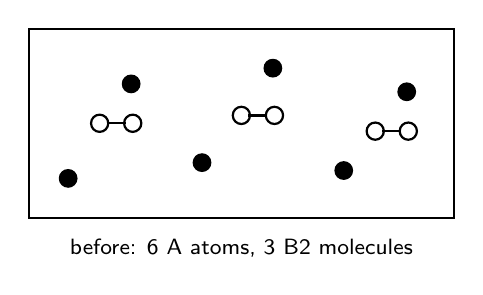
\begin{tikzpicture}[font=\sffamily\footnotesize]
  \draw[thick] (0,0) rectangle (5.4,2.4);
  \foreach \x/\y in {0.5/0.5, 1.3/1.7, 2.2/0.7, 3.1/1.9, 4.0/0.6, 4.8/1.6}
    {\node[circle,fill=black,inner sep=2.4pt] at (\x,\y) {};}
  \foreach \x/\y in {0.9/1.2, 2.7/1.3, 4.4/1.1}
    {\node[circle,draw,thick,inner sep=2.2pt] (a) at (\x,\y) {};
     \node[circle,draw,thick,inner sep=2.2pt] (b) at (\x+0.42,\y) {};
     \draw[thick] (\x+0.09,\y) -- (\x+0.33,\y);}
  \node[below] at (2.7,-0.15) {before: 6 A atoms, 3 \ce{B2} molecules};
\end{tikzpicture}
\end{center}

\begin{parts}
  \item The reaction is \ce{2 A + B2 -> 2 AB}. How many \ce{AB} units form?
        \answerblank[2.4cm]{6}
  \item Which reactant is limiting? \answerblank[4.5cm]{neither --- exact
        ratio}
  \item Draw the ``after'' box. \workspace[3.4cm]
        \keyonly{\begin{apcanswer}6 \ce{AB} units (one filled bonded to one
        open), nothing left over. Atom check: 6 A and 6 B before and
        after.\end{apcanswer}}
\end{parts}

\problem[4.3]{Draw the particulate representation of what is present when
\ce{K2SO4(s)} dissolves in water. Show 3 formula units' worth and label your
symbols; omit water molecules but say so.
\workspace[4cm]
\keyonly{\begin{apcanswer}6 separate \ce{K+} and 3 separate \ce{SO4^2-},
randomly distributed, never drawn as bonded \ce{K2SO4} units. Caption:
``water omitted for clarity.''\end{apcanswer}}}

\problem[4.3]{A student's ``after'' diagram for
\ce{AgNO3(aq) + NaCl(aq) -> AgCl(s) + NaNO3(aq)} shows scattered \ce{Ag+}
and \ce{Cl-} ions plus bonded \ce{NaNO3} pairs. Identify both errors.
\answerlines[3]{\ce{AgCl} is insoluble and must be drawn as a clustered
solid, not free ions. \ce{NaNO3} is soluble and must be drawn as separated
\ce{Na+} and \ce{NO3-}, not bonded pairs. The student has the two products
exactly backwards.}}

\begin{spiralstrip}{Units 1--3 \textbullet\ spiral}
  \item Strongest IMF in \ce{CH3OH}: \answerblank[3.8cm]{hydrogen bonding}
  \item Shape of \ce{NH3}: \answerblank[3.9cm]{trigonal pyramidal}
  \item $PV/nRT<1$ is caused by: \answerblank[3cm]{attractions}
  \item PES areas 2:2:6:1 --- element? \answerblank[2.4cm]{Na}
  \item Moles in \SI{9.0}{\gram} \ce{H2O}: \answerblank[2.6cm]{\SI{0.50}{\mole}}
\end{spiralstrip}

\end{document}
